% CREATED BY DAVID FRISK, 2016
\chapter{Methods}
One of the goals of this thesis was to study how usability tests can be done on teaching materials for teachers, and not just for research studies like this. Therefore, a more generalized methodology was created during the planning of the thesis, and refined as parts of the methodology was tested in practice during the study. Thus, the methodology was both part of the results and part of the method. Because of this, the methods chapter is divided into two parts: First, the methodology is presented, and then the more specific methods used in this thesis are described more in detail.

% When discussing \textit{accessibility} of a teaching material, in this study, it has been separated into two aspects: \textit{obtainability} and \textit{usability}. A method was developed for collecting usability data, but to accomodate for collecting obtainability data, this method was slightly modified when implementing it.
%
%\section{Obtainability}
%Obtainability describes how easy it is for a teacher to obtain a teaching material, and the data for this aspect of accessibility has mainly be acquired through studying literature. Some data connected to obtainability has also been acquired while performing usability testing, partly because these aspect have proven hard to isolate from each other.
%
%\section{Usability}
% The following methodology describes the foundation of the methodology used in this study, as well as a methodology one can use when revising their own shareable teaching material.

\section{The KRUT-methodology}
In the planning phase of this study, a new methodology was developed for usability testing. The methodology was named KRUT, from the processes involved; \textbf{K}ick-off meeting, \textbf{R}evising material, \textbf{U}sability \textbf{T}esting. Developing KRUT helped clarify what the study did and did not aim to investigate and how that was expected to play out. As with ASD, KRUT includes a learning loop. The main purpose of KRUT is to use data collected by usability testing a teaching material to revise said material. Usability testing fills two roles; \textbf{\textit{identifying satisfactory usability}} as well as \textbf{\textit{identifying potential gains in usability}}. KRUT also describes the roles of the different actors, based on the current stage of the testing phase. It is designed with a team of two and a single subject group in mind. The KRUT-methodology is described in figure~\ref{krut}.

\begin{sidewaysfigure}
\centering
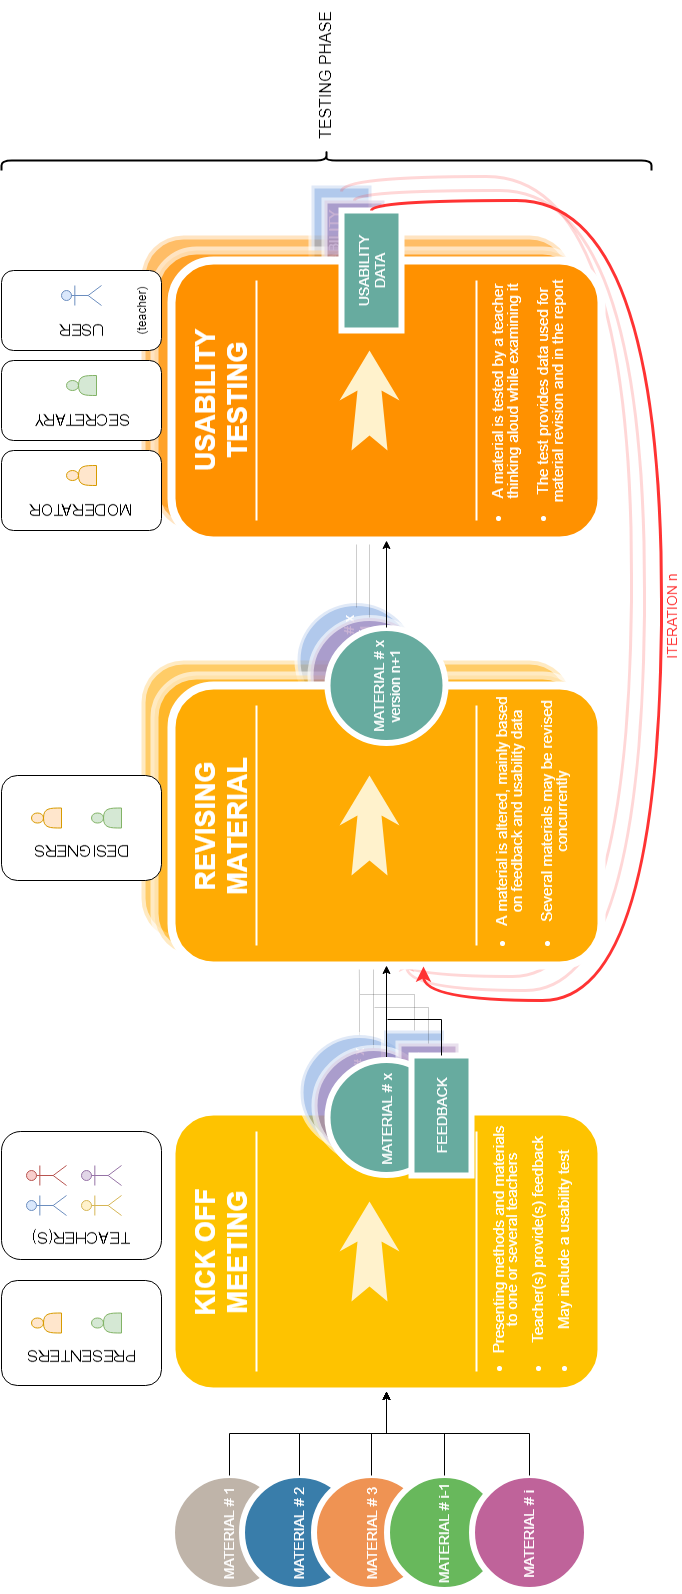
\includegraphics[scale=0.6,angle=-90]{figure/krut.png}
\vspace*{2cm}
\caption{The custom KRUT-methodology, created for usability testing teaching materials}
\label{krut}
\end{sidewaysfigure}

\subsubsection*{Comparing ASD to KRUT} 
There are both similarities and differences when comparing ASD to the KRUT methodology presented in figure~\ref{asd} and figure~\ref{krut}. To compare more easily, KRUT-processes are in bold and ASD-processes are bold-italics. 

The \textbf{Kick Off Meeting} used to introduce one or more teachers to the study, as well as deciding on a teaching material to work on and a date for the first usability test, is comparable to the \textbf{\textit{Project Initiation}} of ASD, being prior to the steps contained inside the \textbf{\textit{Learning Loop}}.

What in the ASD methodology is called \textbf{\textit{Adaptive Cycle Planning}} is the initial step of the \textbf{Revising Material} stage, deciding on how to rework the teaching material based on the data collected from a \textbf{Kick Off Meeting} or previous \textbf{Usability Test}. This is inevitably one of the stages where collected data is summarized and analyzed, even if just as a thought process.

The \textbf{\textit{Concurrent Component Engineering}} part of ASD is practically the same as the \textbf{Revising Material} stage. This is where a coder would revise the code of the program and this is likewise where the product, the teaching material, is being worked on with the intent of improving its usability.

What is called \textbf{\textit{Quality Review}} in ASD is the \textbf{Usability Testing} part of KRUT. This is where the teaching material is tested on a teacher and the data needed to improve the usability of the teaching material is collected. The method used to test usability is based on Steve Krug’s script for usability testing websites. Because a teaching material is quite different from a website, oftentimes focusing on interactivity, the script could not be used without some changes. There is however some important aspects of Steve Krug’s script, e.g. not asking leading questions, that is of great importance to the quality of the data and thereby the quality of future revisions of the teaching material. (Krug, 2010)

The end goal of ASD is called \textbf{\textit{Final QA and Release}}. In the case of KRUT, this step has been reduced. Its original intent is to finalize a product, whereas KRUT defines every revision as an equally valid product, even though the latest revision would theoretically be the most desired.

\section{Implementation of the KRUT methodology in this thesis}
The specific method used in the study differed in certain ways from the metholodogy, for multiple reasons. One of these reasons was that the metholodogy was designed with practical testing in mind rather than scientific testing. Another important reason was that the thesis also studied \textit{obtainability}, while KRUT was mainly designed to test \textit{usability}. Following is a list of details on how specific parts of KRUT were implemented.

\begin{itemize}

\item Obtainability was tested by adding a list of a materials to the test. The test subject picked the teaching material to be tested from the list of materials, which also acted like a usability test of the list itself. The results from this part of the test served as a basis for answering research question 3, about how teachers choose materials.

The list of materials was developed from a list on Kleindagarna's website, which was remade and revised continuously as feedback was collected from the tests.

\item Test subjects consisted of individual teachers and teacher students, instead of a team of teachers. This was mainly due to practical reasons: Individual teachers were easier to find and coordinate than whole teams. This also meant that the Kick Off Meeting was much shorter and done instantly before the test itself.

\item To simplify coordinating the tests, many tests had a single person act as both moderator and secretary during the Usability Testing phase of KRUT. This meant that tests could be done more spontaneously and according to the test subject's needs.

\item A usability testing script was created, see [REFERENS: SCRIPTET], inspired by Krug's script [KÄLLA: KRUGS UT SCRIPT].

\item hehh [N] tests were recorded with video and audio, and [N] tests were recorded by written notes. No tests were transcribed through written notes. Information about the test subject was written down in a template in the test script. More information was recorded than what is recommended when using KRUT for non-scientific reasons, since recorded results are more important in science to make the research more reliable.

\item The revisions of the teaching materials were done in between the tests, but not strictly directly after every test. This is because more revisions were required as the teachers had many different materials to pick from. Doing tests was instead prioritized over doing revisions, and revisions were sometimes postponed in favour of tests. In total, [N] revisions were done.

Another reason for prioritizing tests over revisions was due to revisions initially taking longer than expected. This led to a decision on prioritizing shorter changes and preserving as much of the original material as possible, which shortened time spent per revision significantly.

\end{itemize}

% Test subjects consisted of individual teachers and teacher students, instead of a team (or teams) of teachers, as would have been desired. Because of this, and to collect more data concerning the obtainability aspect, each usability tests began with a stripped down version of a Kick Off Meeting. This meant that the subject was able to choose from a detailed list what teaching material they wanted to use for their usability test. This list was compiled specifically for this study and consisted of teaching materials produced at \todo{mention Kleindagarna earlier or describe more here. /H} Kleindagarna. This was done as a compromise between delimiting the study and offering teaching materials that felt relevant to the teachers. Even though KRUT was designed to be implemented by a team of two, there were no severe difficulties in executing KRUT when the team at times was forced to only one member.

% When revising material, the decisions of what to revise when was determined by a combination of data from usability tests and an analysis of cost versus reward. In practice, this often meant that any usability data that felt intriguing was worth investigating further. It proved to be successful practice to aim for quick changes, rather than trying to rework everything that could be changed at the same time.

\subsection{Result analysis methods}
Analysis of the test results was in two phases: Continuously during every material revision, and once after all tests were finished for the final report. The continuous analysis was done ad-hoc according to the needs of every revision, mostly consisting of summarizing the changes to be done while reading through the usability test notes. The final analysis was done by reading through all the usability test notes and summarizing the findings in a single document, 
  
Since the tests weren't transcribed, there was also some analysis done during each test whenever notes were written. This analysis consisted mostly of interpreting what the test subject said and how they reacted, for example if they reacted confusingly at the material's structure. However, no design decisions were made during this live analysis. Instead, the analysis in the written test notes consisted at most of defining a specific problem in the material, rather than coming up with a solution to the problem. [EXAMPLE?]

\subsection{Test subject anonymity} \label{subjectanonymity}
In this study some personal details were disclosed and some were held anonymous. What is disclosed and examples of what is held anonymous are listed below.

\subsubsection*{Disclosed information}
    \begin{itemize} %Disclosed information
    \item Age – rounded to nearest 5 years.
    \item Current status – if the test subject is currently working as a teacher and if so on what stage of education, or if they are e.g. studying to become a teacher.
    \item Years in teaching – nearest year if under 10 years, can otherwise be rounded to nearest 5 years. No regard to the age of students taught. No regard to full-time or part-time employment.
    \item Subjects – what school subjects is the test subject certified to teach or studying to teach?
\end{itemize}

\subsubsection*{Anonymous information}
\begin{itemize} %Anonymous information
    \item Sex/Gender – the risk of a reader finding false correlations from the data is assumed to be greater if the test subject’s sex and/or gender is disclosed.
    \item Name – the name of the test subjects will not be disclosed, and because the sex/gender will not either, the label of the test subjects will also be as gender free as possible.
    \item Name of school – with this information, it would be too easy to identify the test subject.
    \item Place of school – all subjects studied will live and work in close proximity to Gothenburg, Sweden, as it has been decided to delimit the tests to personal meetings.
\end{itemize}
